% 1986 年全国卷文科第 17 题：圆的直径与三棱锥示意图
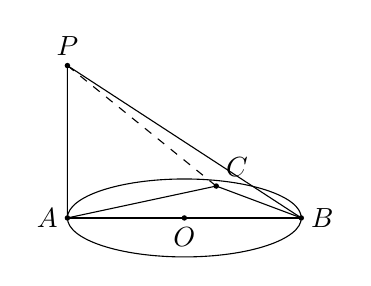
\begin{tikzpicture}[scale=0.9,>=stealth]
  \draw (0,0) ellipse (1.65 and 0.55);
  \draw[dashed] (-1.65,0)--(1.65,0);
  \draw (-1.65,0)--(1.65,0);
  \fill (0,0) circle (1.1pt) node[below] {$O$};
  \fill (-1.65,0) circle (1.1pt) node[left] {$A$};
  \fill (1.65,0) circle (1.1pt) node[right] {$B$};
  \coordinate (C) at (0.45,0.45);
  \fill (C) circle (1.1pt) node[above right] {$C$};
  \coordinate (P) at (-1.65,2.15);
  \fill (P) circle (1.1pt) node[above] {$P$};
  \draw (P)--(-1.65,0);
  \draw (P)--(1.65,0);
  \draw[dashed] (P)--(C);
  \draw (C)--(-1.65,0);
  \draw (C)--(1.65,0);
\end{tikzpicture}
